\documentclass{beamer}
\usepackage{lmodern}
\usepackage{fontspec}
\setmainfont[
  Ligatures=TeX,
  Extension=.otf,
  BoldFont=cmunbx,
  ItalicFont=cmunti,
  BoldItalicFont=cmunbi,
]{cmunrm}
\setsansfont[
  Ligatures=TeX,
  Extension=.otf,
  BoldFont=cmunsx,
  ItalicFont=cmunsi,
]{cmunss}

\usepackage{polyglossia}
\setdefaultlanguage{russian}
\usepackage{amsmath}
\usepackage{graphicx}
\usepackage{subcaption}

\usetheme{Warsaw}
\setbeamertemplate{captionof}[numbered]
\setbeamertemplate{caption}[numbered]

\begin{document}
\title{Проектирование механизма поршневого насоса}  
\author{РК6-53Б, Бригада №3}
\institute{Московский Государственный Технический Университет имени Н.Э. Баумана}
\date{Москва,~\the\year} 
\frame{\titlepage} 

\begin{frame}{Актуальность и цель работы}
    \begin{itemize}
        \item В полевой эксплуатации, при удалённых работах и временном размещении критически важно обеспечить подачу воды,
            в том числе в отдалённые от водных ресурсов места.
        \item Существующие решения имеют \textit{ряд недостатков}:
            \begin{itemize}
                \item зависимость от центральной системы водоснабжения;
                \item громоздкость и низкая мобильность;
                \item недостаточный напор.
            \end{itemize}
        \item \textit{Цель курсовой работы}: проектирование и прототипирование рабочего узла переносного поршневого насоса,
            удовлетворяющего требованиям по мобильности и необходимому напору.
        \item \textit{Пояснение}: под мобильностью понимается максимально допустимая габаритно-весовая характеристика изделия для транспортировки.
    \end{itemize}
\end{frame}

\begin{frame}{Исходные требования и целевые характеристики}
    \begin{itemize}
        \item Проектирование проводится на основе выделенного варианта кривошипно-ползунного механизма.
        \item В качестве идейной основы характеристик конечного изделия использованы требования к умывальнику по СНиП 2.04.01-85.
        \item Целевые характеристики:
            \begin{itemize}
                \item Напор: {{H}} м,
                \item секундный расход воды: {{ (Q * 1000) | round(1) }} л/с,
                \item максимальная плотность жидкости: {{ rho }} кг/$\text{м}^3$,
                \item КПД конструкции: {{ eta_Sigma * 1e+2 }}\%.
                \item КПД объема: {{ eta_v * 1e+2 }}\%.
            \end{itemize}
        \item Гидравлические характеристики:
            \begin{itemize}
                \item Давление: $P = {{ (P_val * 1e-6) | round(6) }}$ МПа.
                \item Полезная мощность: ${{ N_val | round(4)}}$ Вт.
                \item Требуемая мощность: ${{ N_used_val | round(4)}}$ Вт.
            \end{itemize}
    \end{itemize}
\end{frame}

\begin{frame}{Пульсация и выбор многократности}
    \small
    Пульсация -- периодические колебания скорости или расхода жидкости. Для выравнивания подачи используем многократность:
    \centering
    \begin{tabular}{cc}
        
\includegraphics[width=0.45\linewidth]{img/gen/pulse_1.png} &
        
\includegraphics[width=0.45\linewidth]{img/gen/pulse_3.png} \\[6pt]
        
\includegraphics[width=0.45\linewidth]{img/gen/pulse_5.png} &
        
\includegraphics[width=0.45\linewidth]{img/gen/pulse_7.png} \\
    \end{tabular}
    
    \smallskip
    Выбрано 3 цилиндра со сдвигом фаз $120^\circ$: нечётное число даёт более гладкий поток, снижает вибрации; 5–7 цилиндров усложняют конструкцию.
\end{frame}

\begin{frame}{Метрический синтез, кинематическая схема и координаты}
    \tiny
    \begin{figure}
        \centering
        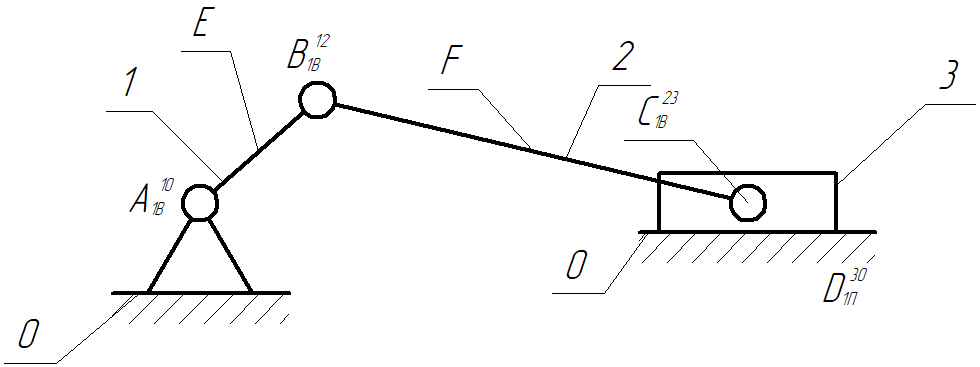
\includegraphics[width=0.65\linewidth]{img/cinematic_schema.png}
        \caption{Кинематическая схема механизма}
    \end{figure}
    Начало системы в точке $A$ (ось кривошипа), $R$ -- длина кривошипа:
    \begin{align*}
        x_{A}(\phi) &= {{ phi_print(ctx['x_A']) }} & y_{A}(\phi) &= {{ phi_print(ctx['y_A']) }}\\
        x_{B}(\phi) &= {{ phi_print(ctx['x_B']) }} & y_{B}(\phi) &= {{ phi_print(ctx['y_B']) }}\\
        x_{C}(\phi) &= {{ phi_print(ctx['x_C']) }} & y_{C}(\phi) &= {{ phi_print(ctx['y_C']) }}\\
        x_{D}(\phi) &= {{ phi_print(ctx['x_D']) }} & y_{D}(\phi) &= {{ phi_print(ctx['y_D']) }}\\
        x_{E}(\phi) &= {{ phi_print(ctx['x_E']) }} & y_{E}(\phi) &= {{ phi_print(ctx['y_E']) }}\\
        x_{F}(\phi) &= {{ phi_print(ctx['x_F']) }} & y_{F}(\phi) &= {{ phi_print(ctx['y_F']) }}\\
    \end{align*}
    Из $x_C(\phi)$ и $x_F(\phi)$ следует $R \le L$.
\end{frame}

\begin{frame}{Скорости и ускорения точек}
    \small
    Скорость — первая производная по $\phi$, ускорение -- вторая производная:
    \centering
    \begin{columns}
        \begin{column}{0.32\textwidth}
            \includegraphics[width=\linewidth]{img/gen/vel_x.png}
            \captionof{figure}{Скорости точек по оси X}
            \includegraphics[width=\linewidth]{img/gen/acc_x.png}
            \captionof{figure}{Ускорения точек по оси X}
        \end{column}
        \begin{column}{0.32\textwidth}
            \includegraphics[width=\linewidth]{img/gen/vel_y.png}
            \captionof{figure}{Скорости точек по оси Y}
            \includegraphics[width=\linewidth]{img/gen/acc_y.png}
            \captionof{figure}{Ускорения точек по оси Y}
        \end{column}
        \begin{column}{0.32\textwidth}
            \includegraphics[width=\linewidth]{img/gen/vel_mod.png}
            \captionof{figure}{Модули скоростей точек}
            \includegraphics[width=\linewidth]{img/gen/acc_mod.png}
            \captionof{figure}{Модули ускорений точек}
        \end{column}
    \end{columns}
    \begin{tabular}{ccc}
    \end{tabular}
    
    \smallskip
    Длины звеньев: $R = {{ (R_val * 1000) | int}}$ мм, $L = {{ (L_val * 1000) | int }}$ мм, $S = 2R = {{ (S_val * 1000) | int }}$ мм.
\end{frame}

{% set d_M = diff('R*F*(sin(phi(t))*(sqrt(L^2 - (R*sin(phi(t)))^2)/L) + cos(phi(t)) * (R*sin(phi(t))/L))', 'phi(t)') -%}
{% set phi_M_max = solve_for_0(diff(with_var_phi(M_A_val), phi_symb), phi_symb, 0, 2*pi, 0.001) -%}
{% set M_max = (as_fun('phi', with_var_phi(M_A_val))(phi_M_max)) -%}
{% set F_BC_max = as_fun('phi', with_var_phi(F_BC_val))(pi/2) -%}
\begin{frame}{Силовой расчёт, опасные положения и реакции}
    \small
    Квазистатический анализ, сила сопротивления жидкости на поршень: $F = P \cdot A = {{ (F_val) | round(3) }}\ \text{Н}$
    \begin{columns}
        \begin{column}{0.5\textwidth}
            \begin{block}{Максимальные силы}
                \tiny
                \begin{align*}
                    \textbf{Кривошип:} &\phi = {{ phi_M_max | round(4) }} \text{рад,}\\ 
                    & M_{\max}= {{ M_max | round(4) }}\ \text{Н $\cdot$ м} \\
                    \textbf{Шатун:} &\phi = \frac{\pi}{2}, \\
                    & F_{BC_{max}} = {{ F_BC_max | round(3) }}\ \text{Н}
                \end{align*}
            \end{block}
        \end{column}
        \begin{column}{0.5\textwidth}
            \centering
            \includegraphics[width=\linewidth]{img/gen/reactions_A.png} \\
            \captionof{figure}{Реакции в точке A}
        \end{column}
    \end{columns}
    
    \begin{columns}
        \begin{column}{0.5\textwidth}
            \centering
            \includegraphics[width=\linewidth]{img/gen/reactions_B.png} \\
            \captionof{figure}{Реакции в точке B}
        \end{column}
        \begin{column}{0.5\textwidth}
            \centering
            \includegraphics[width=\linewidth]{img/gen/reactions_C.png} \\
            \captionof{figure}{Реакции в точке C}
        \end{column}
    \end{columns}
\end{frame}

\begin{frame}{Эпюры}
    \begin{columns}
        \begin{column}{0.5\textwidth}
            \centering
            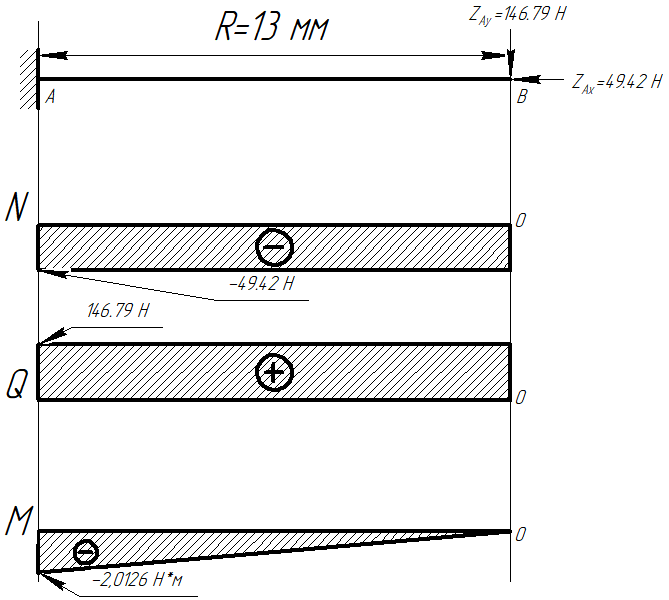
\includegraphics[width=\linewidth]{img/crank_schema.png} \\
            \captionof{figure}{Эпюра кривошипа}
        \end{column}
        \begin{column}{0.5\textwidth}
            \centering
            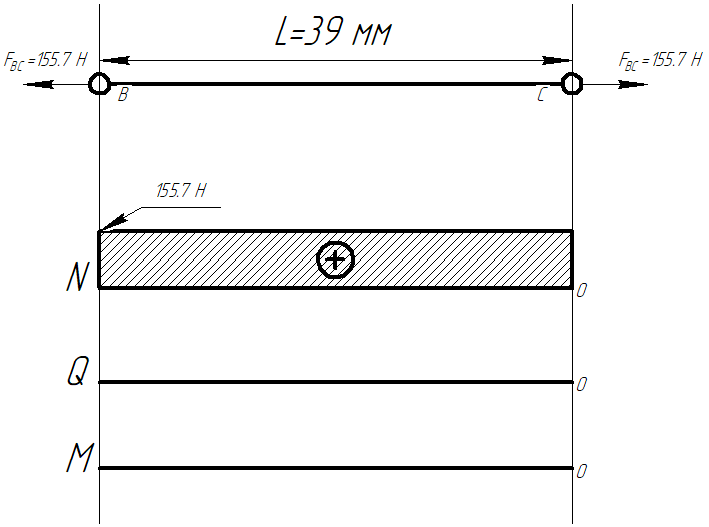
\includegraphics[width=\linewidth]{img/rod_schema.png} \\
            \captionof{figure}{Эпюра шатуна}
        \end{column}
    \end{columns}
\end{frame}

\begin{frame}{Подбор материала}
    \small
    Принятые сечения:
    \begin{itemize}
        \item ползун: $d=19.05\ \text{мм},\quad A_p={{ (with_d(A_p_val) * 1e+6) | round(3)}} \text{мм}^2$;
        \item кривошип/шатун: квадрат $d_r=5\ \text{мм},\quad A_r={{ (with_d(A_r_val) * 1e+6) | round(3)}} \text{мм}^2$.
    \end{itemize}
    
    {% set sQ_crank = as_fun('phi', with_var_phi(sigma_Q_crank_val))(phi_M_max) -%}
    {% set sN_crank = as_fun('phi', with_var_phi(sigma_N_crank_val))(phi_M_max) -%}
    {% set sM_crank = as_fun('phi', with_var_phi(sigma_M_crank_val))(phi_M_max) -%}
    {% set s_crank = sN_crank + sM_crank + sQ_crank -%}
    {% set sN_rod = as_fun('phi', with_var_phi(sigma_N_rod_val))(pi/2) -%}
    {% set sQ_rod = as_fun('phi', with_var_phi(sigma_Q_rod_val))(pi/2) -%}
    {% set s_rod = sN_rod + sQ_rod -%}
    
    Оценочные напряжения:
    \[
    \sigma_{c}\approx {{ (s_crank * 1e-6) | round(3) }}\ \text{МПа},\qquad
    \sigma_{r}\approx {{ (s_rod * 1e-6) | round(3) }}\ \text{МПа}
    \]
    
    Выбор материала: «Сталь 40 (ГОСТ 1050-2013)», $\sigma_{T}\approx335\ \text{МПа}$,
    с учетом запаса $[\sigma]\approx {{ (1e-6*s_crank * 2.2) | round(2) }}\ \text{МПа}$ -- хватает с запасом.
    Материал: «Сталь 40», $\rho_{mat} = {{ rho_m }}$. Массы: $m = \rho_{mat}A\ell$.
    \begin{align*}
        & m_1={{ (with_d(m_1_val) * 1e+2) | round(3) }}\cdot 10^{-2}\ \text{кг}, \quad
        m_2={{ (with_d(m_2_val) * 1e+2) | round(3) }}\cdot 10^{-2}\ \text{кг}, \quad
        m_3={{ (with_d(m_3_val) * 1e+2) | round(3) }}\cdot 10^{-2}\ \text{кг}.
    \end{align*}
\end{frame}

\begin{frame}{Проверка влияния инерции}
    \small
    {% set I_3x_0 = af(I_3x_val)(0) -%}
    {% set I_2x_max = af(I_2x_val)(0) -%}
    {% set I_2y_max = af(I_2y_val)(pi/2) -%}
    {% set I_1_max = af(I_1_val)(0) -%}
    \begin{block}{Инерционные силы}
    \begin{itemize}
        \item $|F^{\,\text{ин}}_{3x}|_{\max}\approx {{ abs(I_3x_0) | round(3) }} \ \text{Н}$,
        \item $|F^{\,\text{ин}}_{2x}|_{\max}\approx {{ abs(I_2x_max) | round(3) }} \ \text{Н}$,
        \item $|F^{\,\text{ин}}_{2y}|_{\max}\approx {{ abs(I_2y_max) | round(3) }} \ \text{Н}$.
    \end{itemize}
    \end{block}
    \begin{alertblock}{Влияние на нагрузку}
    Вклад в основную нагрузку $F={{ F_val | round(3) }}\ \text{Н}$: порядка $0.1\ldots1.5\%$.
    \end{alertblock}
    {% set mI_3x_max = abs_max(I_3x_val) -%}
    {% set mI_2x_max = abs_max(I_2x_val) -%}
    {% set mI_2y_max = abs_max(I_2y_val) -%}
    {% set mI_1x_max = abs_max(I_1x_val) -%}
    {% set mI_1y_max = abs_max(I_1y_val) -%}
    {% set mI_1_max = abs_max(I_1_val) -%}
    {% set DZ_Cy = (mI_1_max + mI_2y_max) -%}
    {% set DZ_C = sqrt(mI_3x_max**2 + DZ_Cy**2) -%}
    {% set DZ_Ax = (mI_1x_max + mI_2x_max + mI_3x_max)-%}
    {% set DZ_A = sqrt(DZ_Ax**2 + DZ_Cy**2) -%}
    {% set DM_A = R_val * (mI_2x_max + mI_3x_max + mI_2y_max ) + af(J_2_eps_val)(pi/2) -%}
    {% set k_M = (M_max + DM_A)/M_max -%}
    {% set k_Z_A = (F_BC_max + DZ_A)/F_BC_max -%}
    {% set k_Z_C = (F_BC_max + DZ_C)/F_BC_max -%}
    
    \begin{block}{Изменения в нагрузке с учетом инерционных сил}
    \[
    k_M\lesssim {{k_M | round(3)}},\quad
    k_{Z_A}\lesssim {{ k_Z_A | round(3)}},\quad
    k_{Z_C}\lesssim {{ k_Z_C | round(3)}}.
    \]
    $k_{max}\approx 1.007 < n_{\min}=2.2$ — учёт инерции не выводит расчёт за пределы запаса прочности.
    \end{block}
\end{frame}

\begin{frame}{Конструкторский этап}
    \small
    Была составлена базовая модель согласно расчетам, проведенными в работе.
    \begin{alertblock}{Неудача}
        Базовая модель, изготовленная с помощью технологии 3Д-печати, показала себя недостаточно прочной
        и потребовала конструкционных изменений.
    \end{alertblock}
    \begin{tabular}{ccc}
        \centering
        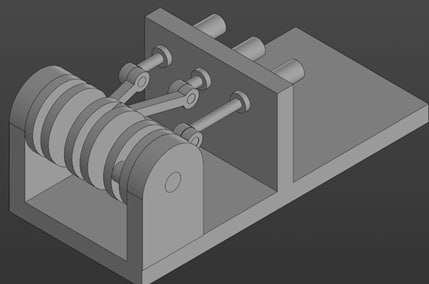
\includegraphics[width=0.3\linewidth]{img/base_model/iso_main.jpg} &
        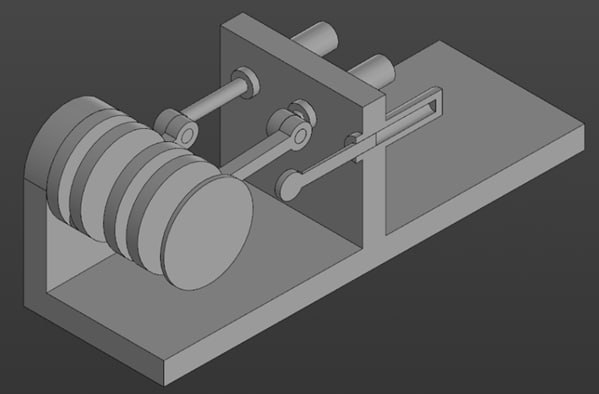
\includegraphics[width=0.3\linewidth]{img/base_model/iso_back.jpg} &
        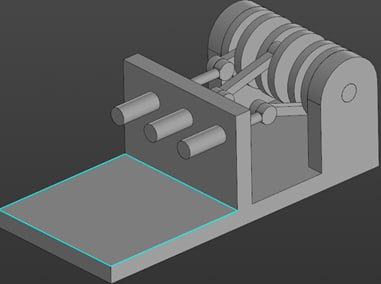
\includegraphics[width=0.3\linewidth]{img/base_model/iso_side.jpg} \\
        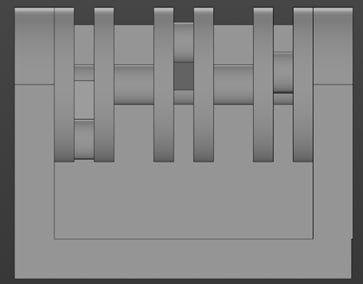
\includegraphics[width=0.3\linewidth]{img/base_model/back.jpg} &
        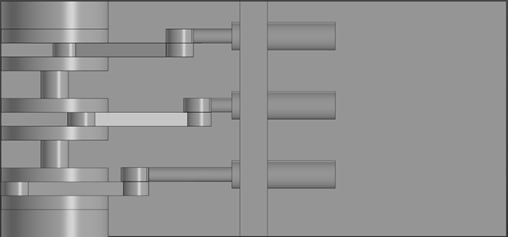
\includegraphics[width=0.3\linewidth]{img/base_model/up.jpg} &
        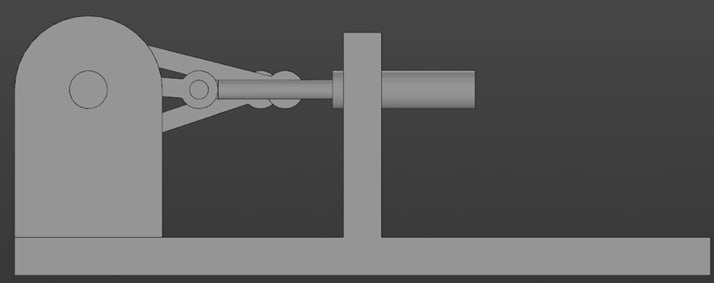
\includegraphics[width=0.3\linewidth]{img/base_model/side.jpg} \\
    \end{tabular}
\end{frame}

\begin{frame}{Финальная модель}
    \small
    \begin{block}{Адаптация под пластик}
        Для оптимизации прототипа под 3Д-печать, были внесены некоторые изменения для увеличения прочности
        прототипа с учетом особенностей рабочего материала
    \end{block}
    \centering
    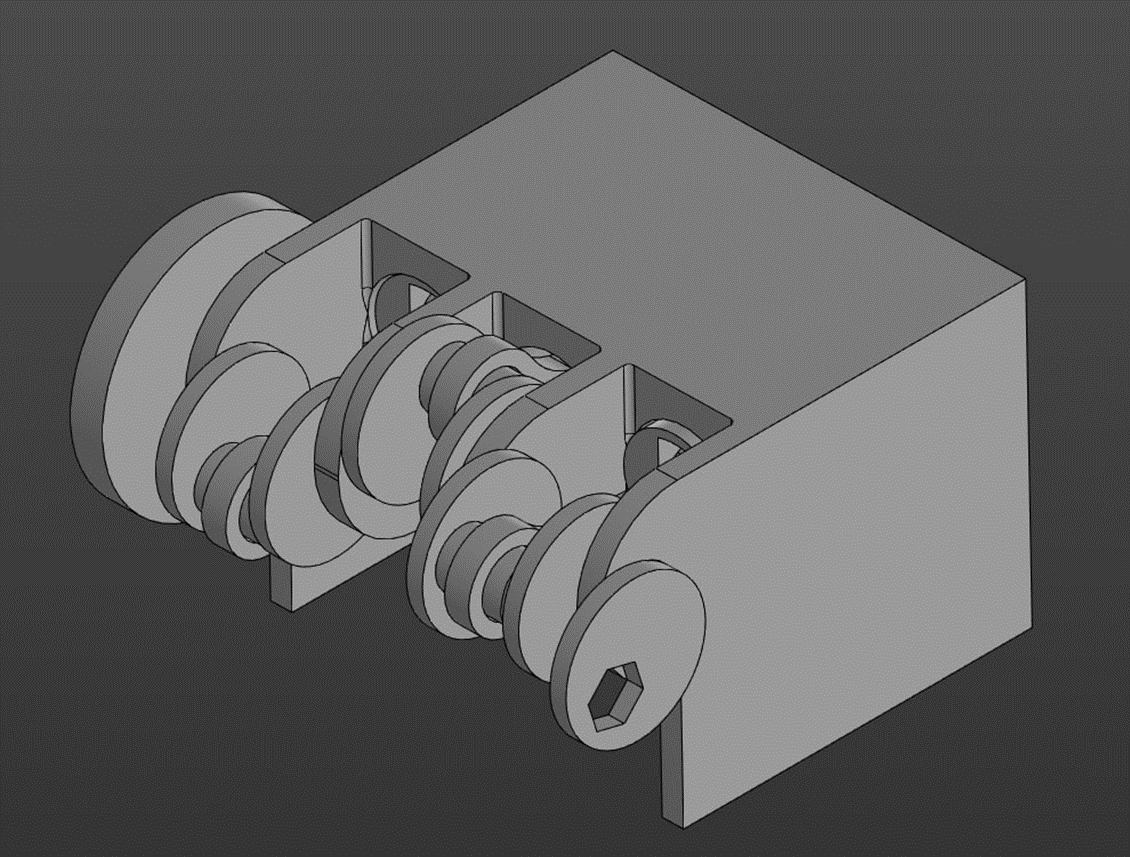
\includegraphics[width=0.5\linewidth]{img/final_model.png}
    \captionof{figure}{Финальная модель прототипа, адаптированная под 3Д-печать}
\end{frame}

\begin{frame}{Метод конечных элементов (МКЭ)}
    \small
    Расчёт звеньев методом конечных элементов для проверки нагрузки и укрепления слабых точек.
    Предел текучести «Сталь 40 ГОСТ 1050-2013»: $\sigma_m \approx 335\ \text{МПа}$.
    
    \begin{columns}
        \begin{column}{0.5\textwidth}
            \centering
            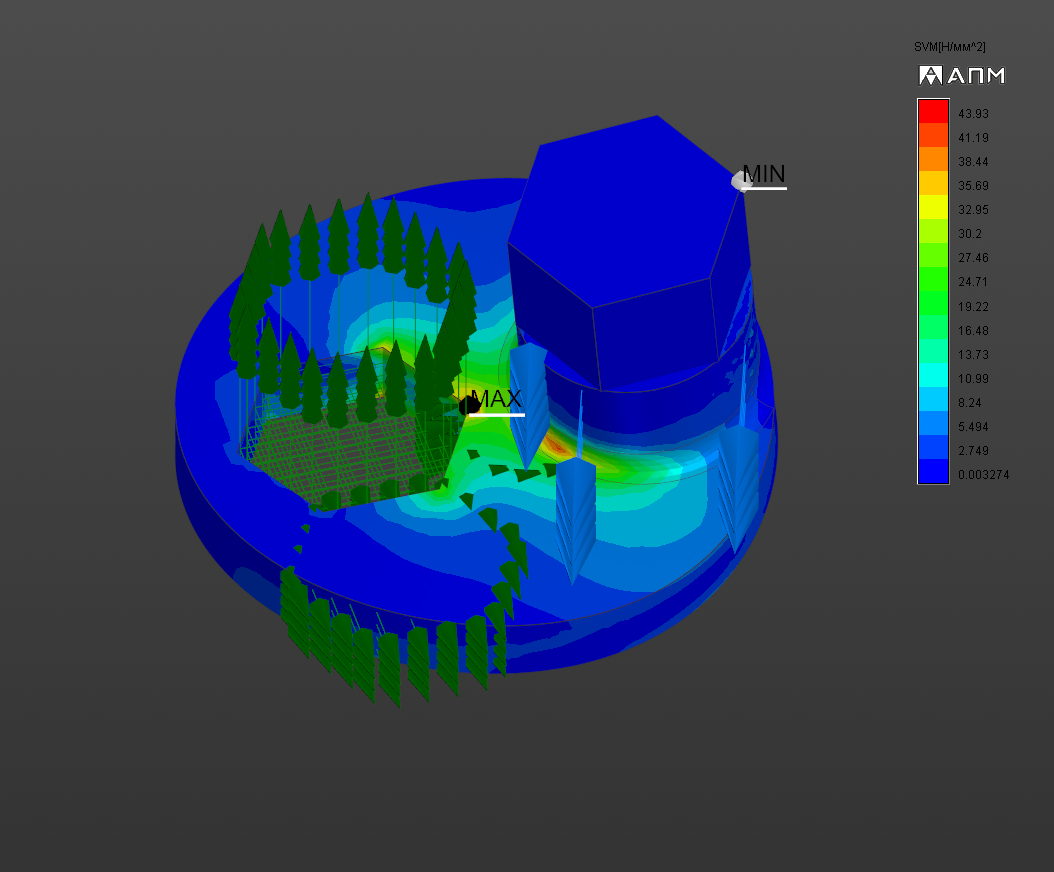
\includegraphics[width=0.6\linewidth]{img/mke/crank_stress.png} \\
            \captionof{figure}{Кривошип: напряжения}
        \end{column}
        \begin{column}{0.5\textwidth}
            \centering
            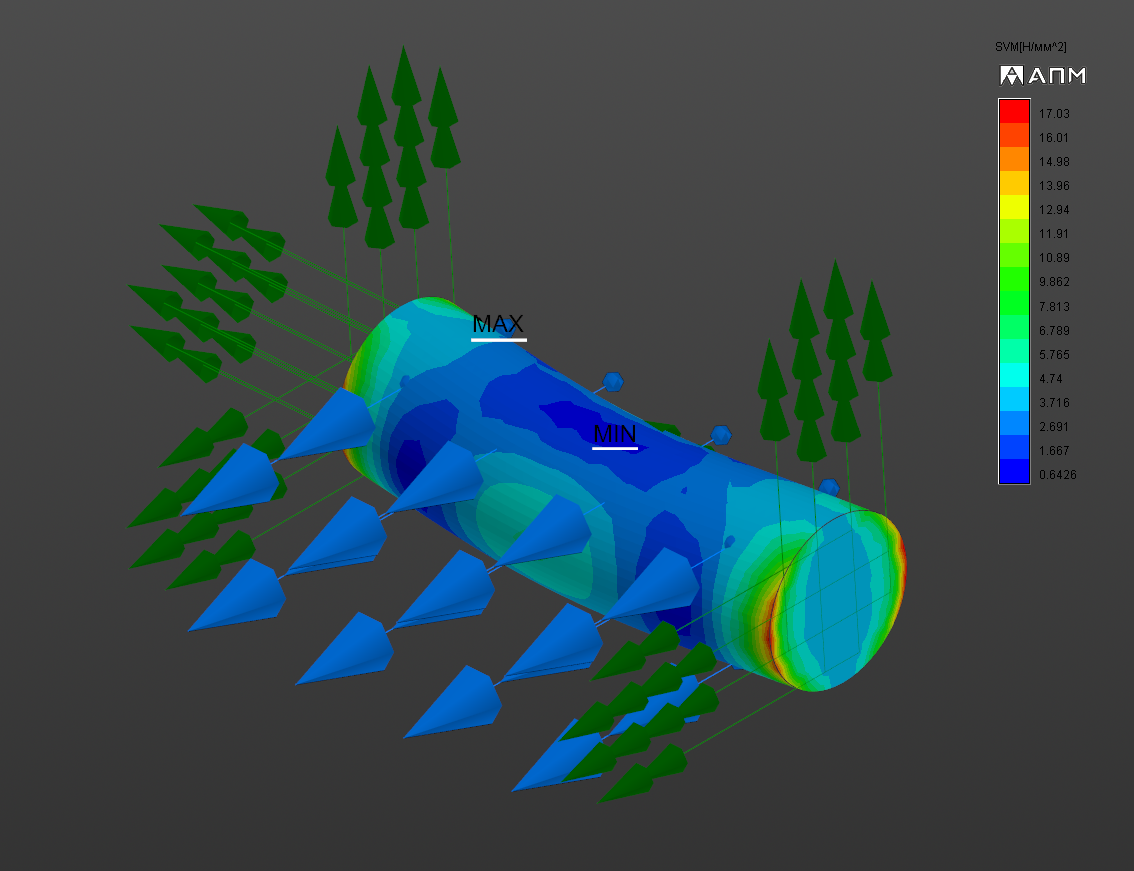
\includegraphics[width=0.6\linewidth]{img/mke/finger_stress.png} \\
            \captionof{figure}{Палец: напряжения}
        \end{column}
    \end{columns}
    
    \begin{columns}
        \begin{column}{0.5\textwidth}
            \centering
            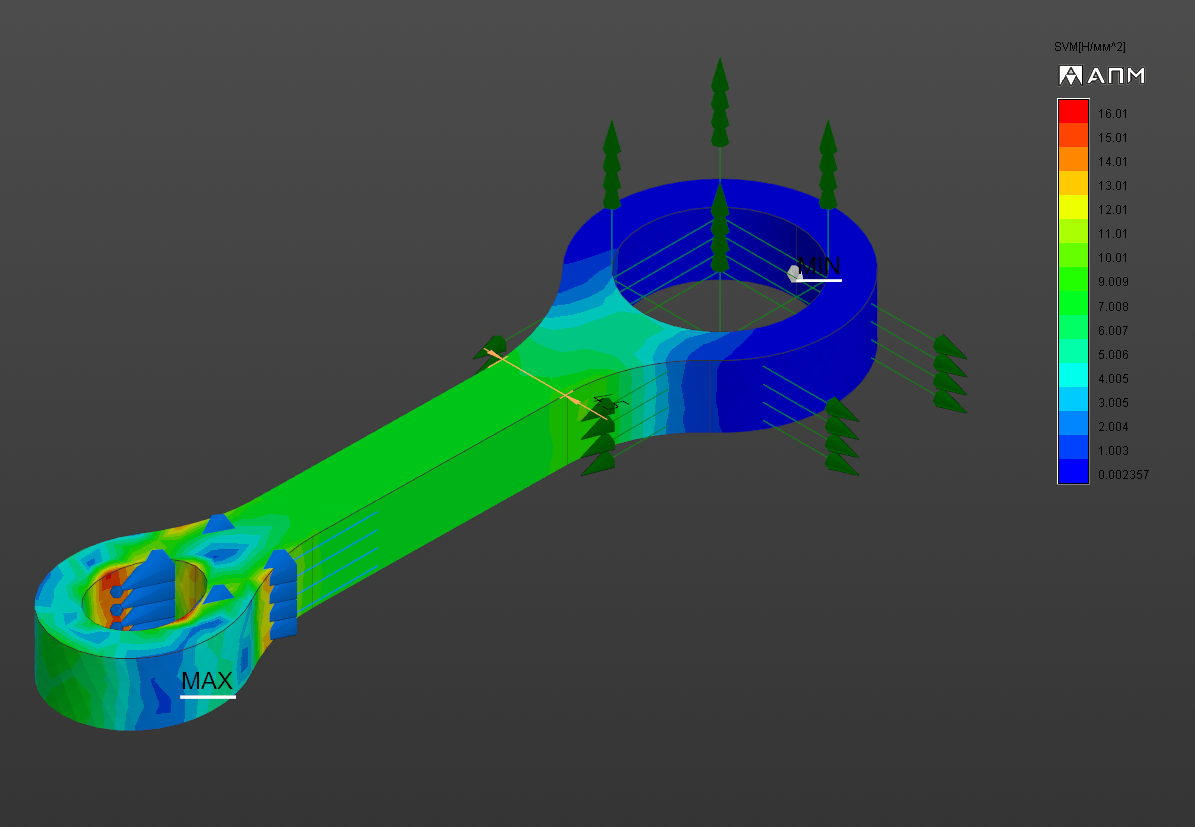
\includegraphics[width=0.6\linewidth]{img/mke/r2p_stress.png} \\
            \captionof{figure}{Шатун (со стороны кривошипа)}
        \end{column}
        \begin{column}{0.5\textwidth}
            \centering
            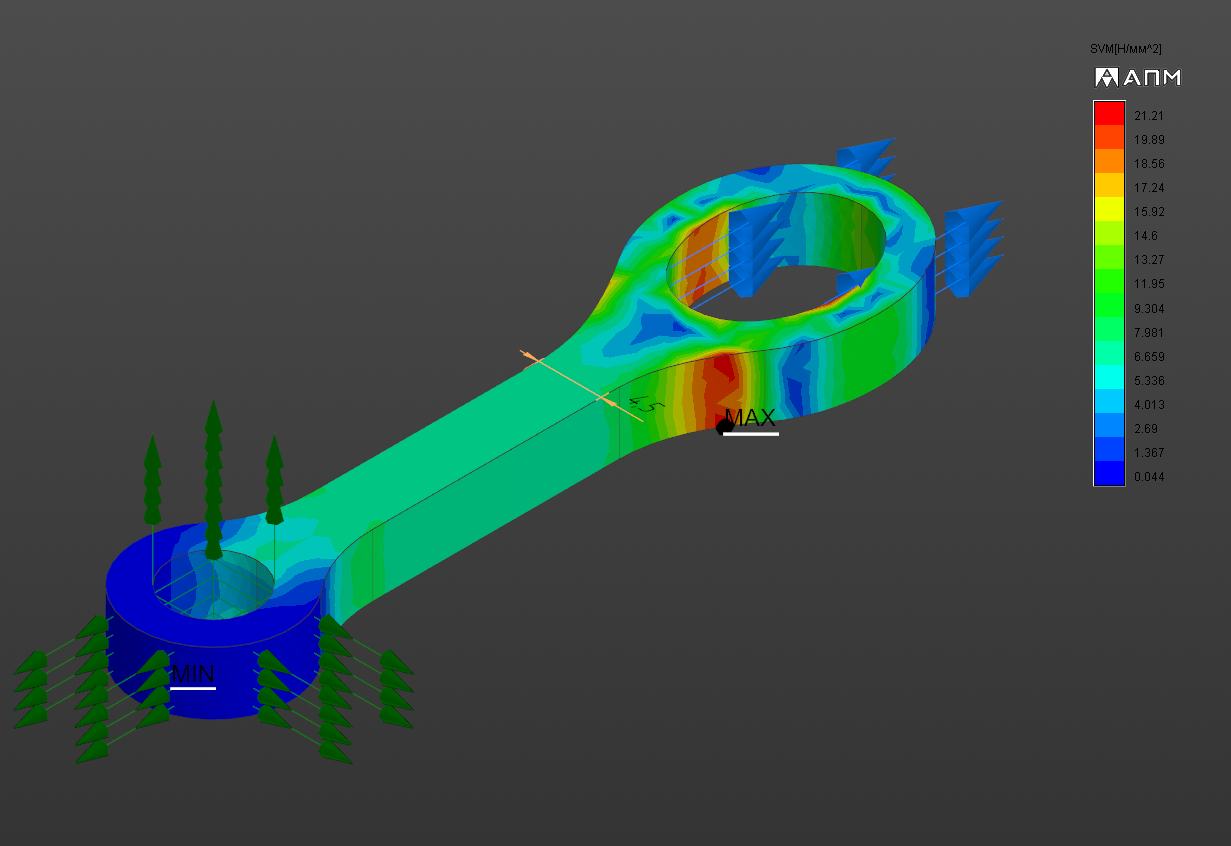
\includegraphics[width=0.6\linewidth]{img/mke/p2r_stress.png} \\
            \captionof{figure}{Шатун (со стороны ползуна)}
        \end{column}
    \end{columns}
\end{frame}

\begin{frame}{МКЭ -- перемещения}
    \small
    \begin{columns}
        \begin{column}{0.5\textwidth}
            \centering
            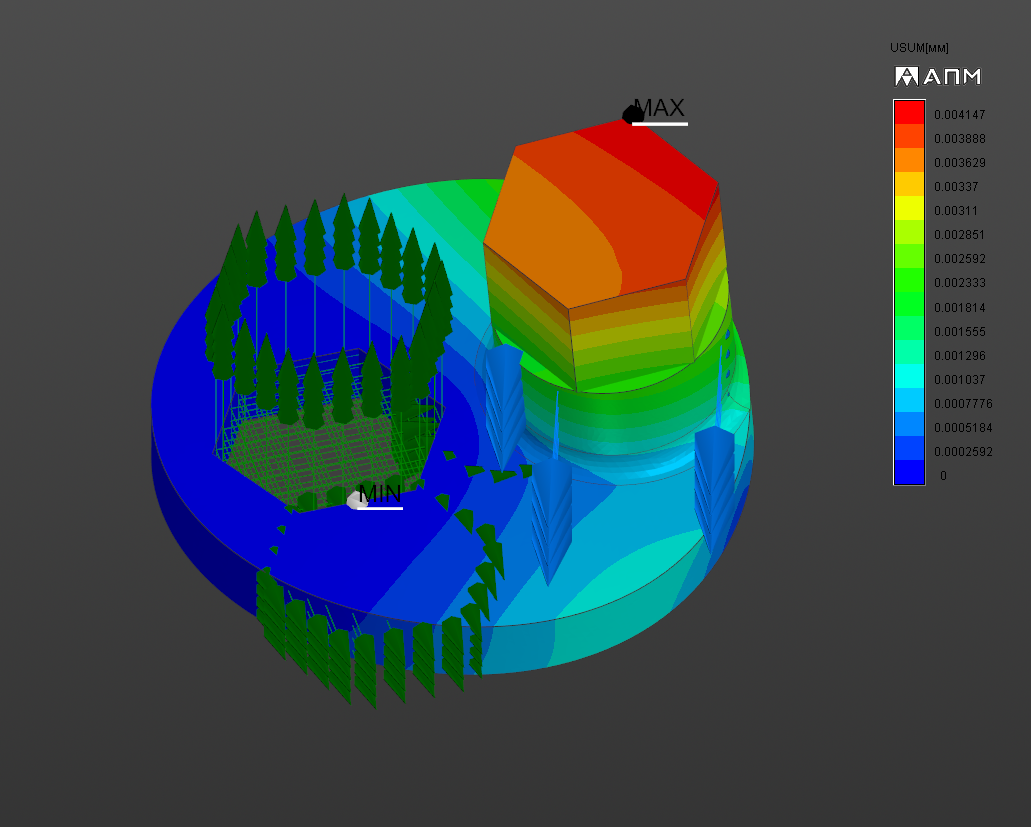
\includegraphics[width=0.6\linewidth]{img/mke/crank_shift.png} \\
            \captionof{figure}{Кривошип: перемещения}
        \end{column}
        \begin{column}{0.5\textwidth}
            \centering
            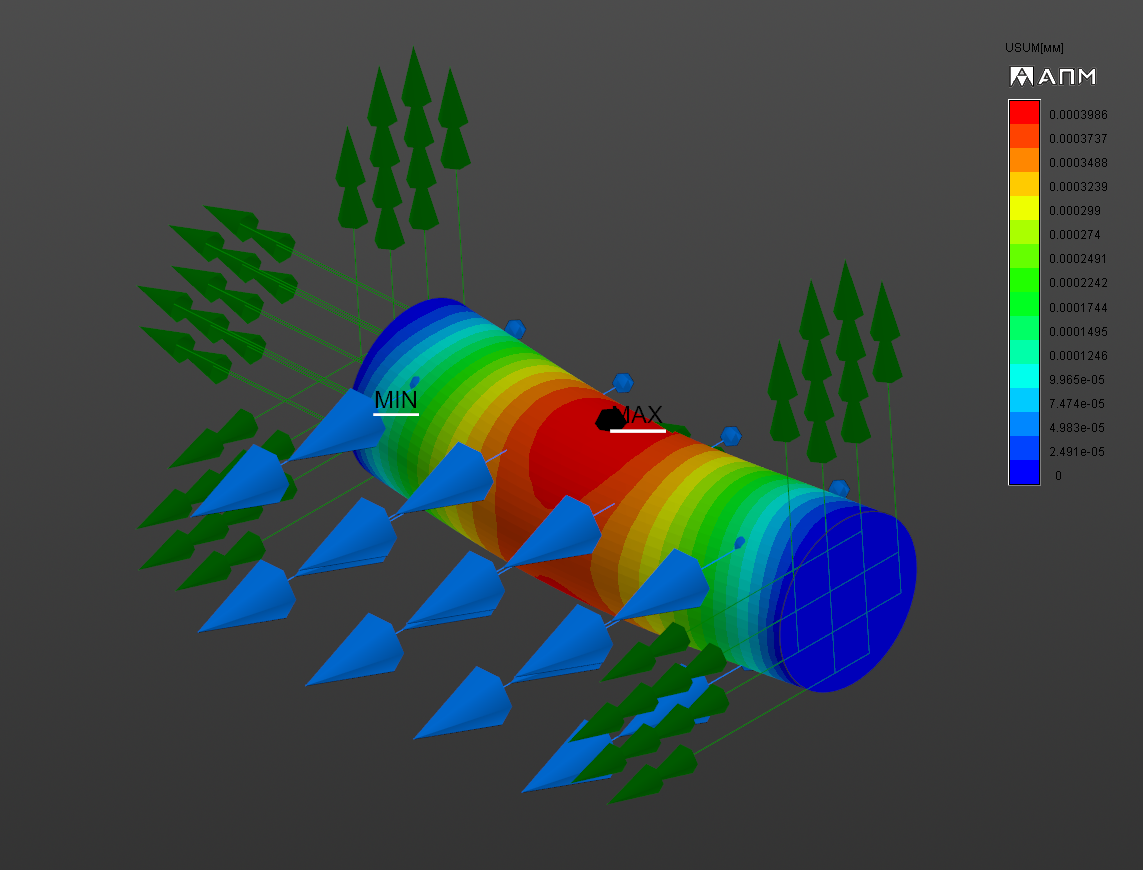
\includegraphics[width=0.6\linewidth]{img/mke/finger_shift.png} \\
            \captionof{figure}{Палец: перемещения}
        \end{column}
    \end{columns}
    
    \begin{columns}
        \begin{column}{0.5\textwidth}
            \centering
            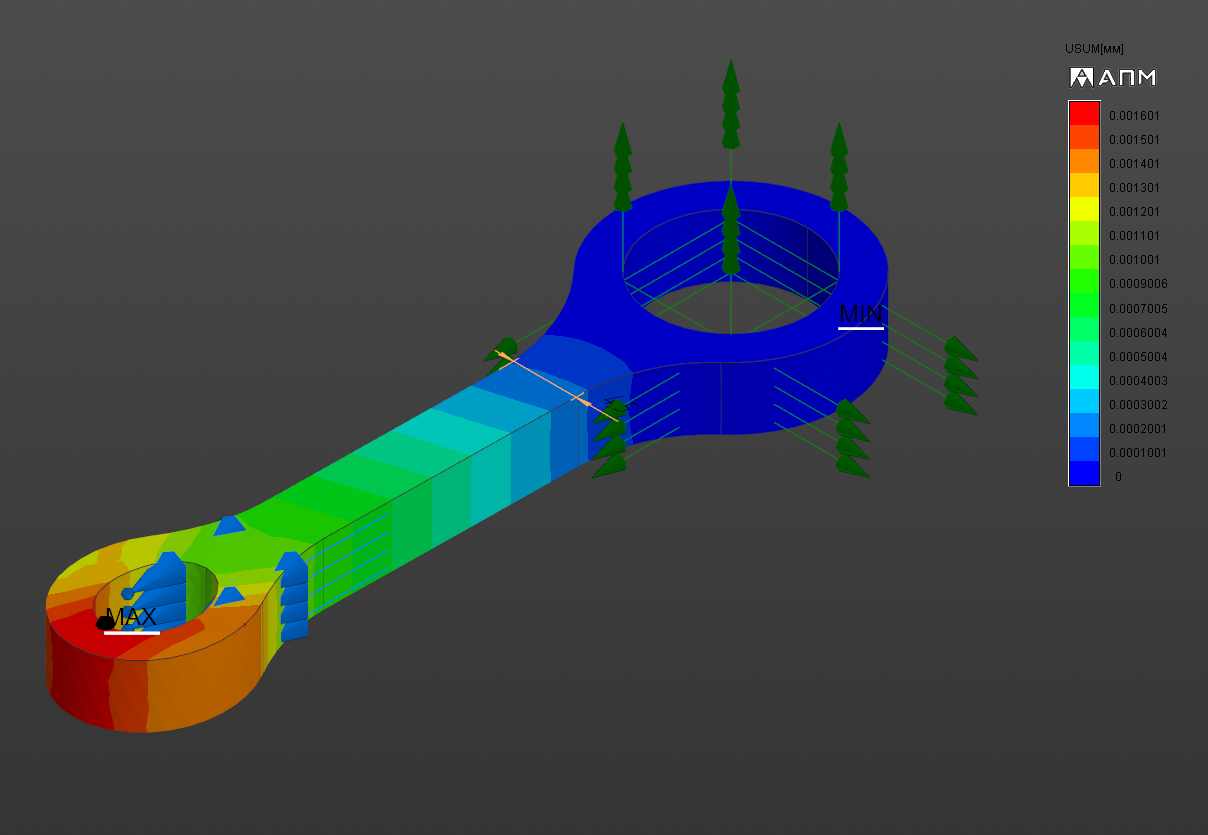
\includegraphics[width=0.6\linewidth]{img/mke/r2p_shift.png} \\
            \captionof{figure}{Шатун (со стороны кривошипа)}
        \end{column}
        \begin{column}{0.5\textwidth}
            \centering
            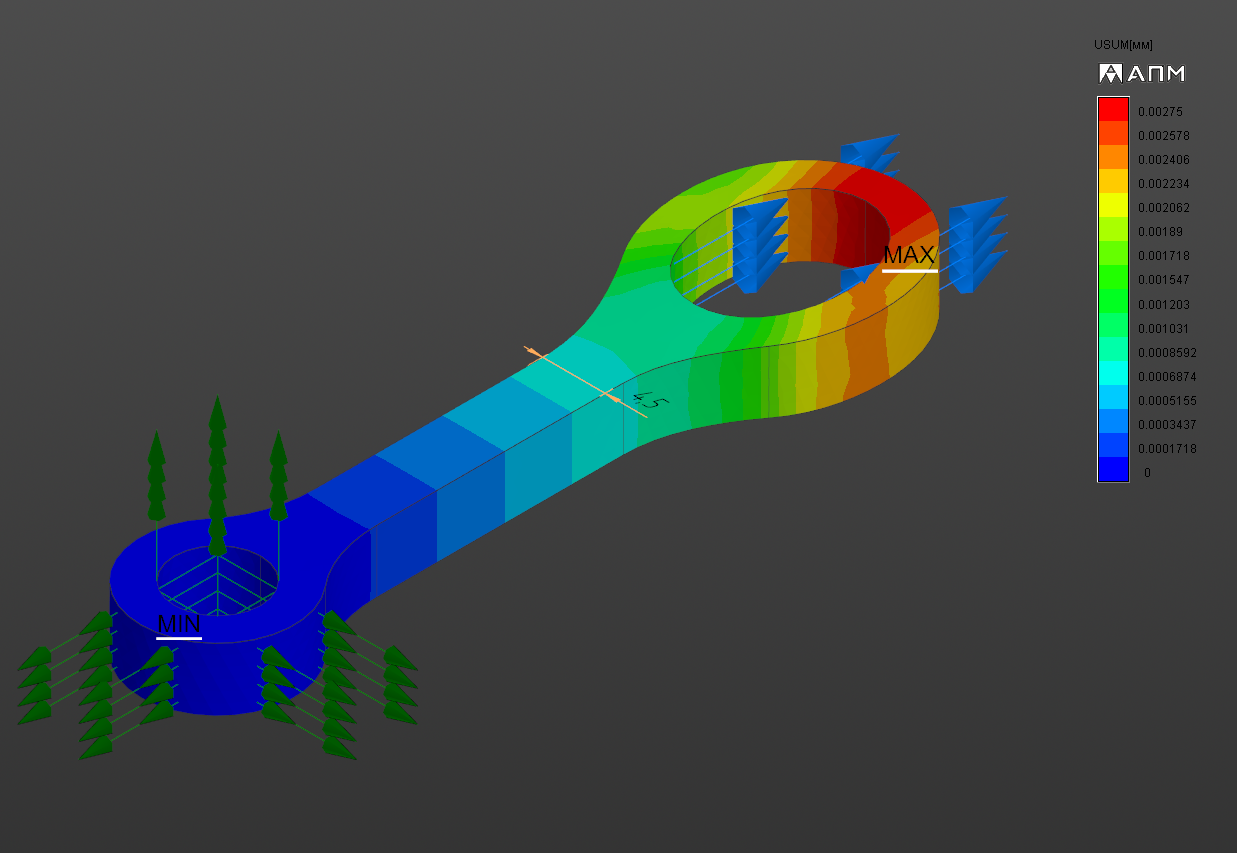
\includegraphics[width=0.6\linewidth]{img/mke/p2r_shift.png} \\
            \captionof{figure}{Шатун (со стороны ползуна)}
        \end{column}
    \end{columns}
\end{frame}

\begin{frame}{Итоги}
    \tiny
\begin{enumerate}
    \item Проведён расчёт исходных гидравлических параметров: по заданным $Q$, $\rho$, $H$ определено давление
        $P\approx {{ (1e-6 * P_val) | round(6) }} \text{ МПа}$ и полезная мощность
        $N_{\text{used}}\approx {{N_val | round(3)}} \text{ Вт}$; с учётом суммарного КПД $\eta_{\Sigma}={{eta_Sigma}}$
        обоснована требуемая мощность электропривода порядка {{N_used_val | round(3)}} Вт.
    \item Рассмотрена неравномерность подачи поршневого насоса и выбран способ её снижения:
        применена многократность — три цилиндра параллельно со сдвигом фаз $120^\circ$, что по расчётной оценке существенно
        уменьшает пульсацию расхода по сравнению с одиночным цилиндром.
    \item Выполнены метрический синтез и кинематический анализ кривошипно-ползунного механизма:
        получены уравнения движения характерных точек, определены скорости и ускорения, что обеспечило исходную базу для силовых расчётов.
    \item Проведён первичный (квазистатический) силовой анализ: получены зависимости приводного момента $M_A(\phi)$
        и реакций в опоре $Z_A(\phi)$ и шарнире $Z_C(\phi)$, выявлены интервалы, в которых из-за режима простого действия
        часть нагрузки воспринимается одним цилиндром.
    \item Выполнен прочностной расчёт звеньев в плоской постановке (кривошип и шатун): определены опасные положения и опасные сечения
        (для кривошипа — у заделки в точке $A$, для шатуна — минимальное рабочее сечение), рассчитаны напряжения,
        показано выполнение условия прочности при выборе материала "Сталь 40 ГОСТ 1050-2013" с существенным запасом.
    \item Проведён уточнённый силовой анализ с учётом сил инерции по методу Д’Аламбера: оценены массы звеньев и инерционные составляющие,
        установлено, что их вклад в основные силовые факторы составляет порядка $0.1\ldots1.5\%$, а в приводной момент — порядка нескольких процентов.
    \item Выполнена проверка применимости квазистатического расчёта: консервативно показано,
        что изменение максимумов $M_A$, $Z_A$, $Z_C$ при учёте инерции не превышает $\sim 0.7\%$,
        что существенно меньше принятого коэффициента запаса $n_\text{запаса}=2.2$; следовательно, принятые расчётные зависимости
        являются обоснованными для дальнейшего проектирования.
    \item На конструкторской стадии разработаны 3D-модели механизма (первичная и базовая),
        выполнена корректировка компоновки (дисковый/сборный коленвал, переработка узлов разборности и соединений),
        а также проведён МКЭ-анализ звеньев с последующей модификацией геометрии для снижения концентраций напряжений
        (скругления и сглаживания кромок в наиболее нагруженных зонах).

\end{enumerate}
\end{frame}

\end{document}
